%%%%%%%%%%%%%%%%%%%%%%%%%%%%%%%%%%%%%%%%%
% Journal Article
% LaTeX Template
% Version 1.3 (9/9/13)
%
% This template has been downloaded from:
% http://www.LaTeXTemplates.com
%
% Original author:
% Frits Wenneker (http://www.howtotex.com)
%
% License:
% CC BY-NC-SA 3.0 (http://creativecommons.org/licenses/by-nc-sa/3.0/)
%
%%%%%%%%%%%%%%%%%%%%%%%%%%%%%%%%%%%%%%%%%

%----------------------------------------------------------------------------------------
%	PACKAGES AND OTHER DOCUMENT CONFIGURATIONS
%----------------------------------------------------------------------------------------

\documentclass{article}

%\usepackage{lipsum} % Package to generate dummy text throughout this template

%\usepackage[sc]{mathpazo} % Use the Palatino font
\usepackage{amsmath}
\usepackage[T1]{fontenc} % Use 8-bit encoding that has 256 glyphs
\linespread{1.05} % Line spacing - Palatino needs more space between lines
\usepackage{microtype} % Slightly tweak font spacing for aesthetics

\usepackage[hmarginratio=1:1,top=32mm,columnsep=20pt]{geometry} % Document margins
\usepackage{multicol} % Used for the two-column layout of the document
\usepackage[hang, small,labelfont=bf,up,textfont=it,up]{caption} % Custom captions under/above floats in tables or figures
%\usepackage{booktabs} % Horizontal rules in tables
\usepackage{float} % Required for tables and figures in the multi-column environment - they need to be placed in specific locations with the [H] (e.g. \begin{table}[H])
\usepackage{hyperref} % For hyperlinks in the PDF

\usepackage{lettrine} % The lettrine is the first enlarged letter at the beginning of the text
%\usepackage{paralist} % Used for the compactitem environment which makes bullet points with less space between them

\usepackage{abstract} % Allows abstract customization
\renewcommand{\abstractnamefont}{\normalfont\bfseries} % Set the "Abstract" text to bold
\renewcommand{\abstracttextfont}{\normalfont\small\itshape} % Set the abstract itself to small italic text

%\usepackage{float}% Places a thin box around figures
%\floatstyle{boxed} 
%\restylefloat{figure}
\usepackage{graphicx}


%\usepackage{titlesec} % Allows customization of titles
%\renewcommand\thesection{\Roman{section}} % Roman numerals for the sections
%\renewcommand\thesubsection{\Roman{subsection}} % Roman numerals for subsections
%\titleformat{\section}[block]{\large\scshape\centering}{\thesection.}{1em}{} % Change the look of the section titles
%\titleformat{\subsection}[block]{\large}{\thesubsection.}{1em}{} % Change the look of the section titles

\usepackage{fancyhdr} % Headers and footers
\pagestyle{fancy} % All pages have headers and footers
\fancyhead{} % Blank out the default header
\fancyfoot{} % Blank out the default footer
\fancyhead[C]{Heavy Photon Search Collaboration Note \#2018-001} % Custom header text
\fancyfoot[RO,LE]{\thepage} % Custom footer text

\newcommand{\gev}{GeV~}
\newcommand{\mev}{MeV~}

\newcommand{\gevcc}{GeV/c$^2$}
\newcommand{\mevcc}{MeV/c$^2$}
\newcommand{\ap}{A^\prime}
\newcommand{\pos}{e^+}
\newcommand{\ele}{e^-}
\newcommand{\trifull}{\ele~W\to\ele\ele\pos~W}
\newcommand{\apfull}{\ele~W\to\ele\ap(\to\ele\pos)~W}
\newcommand{\epem}{\pos\ele}




%----------------------------------------------------------------------------------------
%	TITLE SECTION
%----------------------------------------------------------------------------------------

\title{\vspace{-15mm}\fontsize{24pt}{10pt}\selectfont\textbf{Comparison of MC cross-sections for Radiative and Bethe-Heitler  trident production obtained from MadGraph5 and CalcHep}} % Article title
\author{
\large
\textsc{Andrea Celentano}\\ % Your name
\normalsize INFN-Genova\\ % Your institution
\normalsize \href{mailto:andrea.celentano@ge.infn.it}{andrea.celentano@ge.infn.it} % Your email address
\vspace{0mm}
}
\date{\today}

%----------------------------------------------------------------------------------------

\begin{document}


\maketitle % Insert title

\thispagestyle{fancy} % All pages have headers and footers

%----------------------------------------------------------------------------------------
%	ABSTRACT
%----------------------------------------------------------------------------------------

\begin{abstract}
We compare the results obtained from MadGraph5 and CalcHep codes in the calculation of the cross-sections for radiative and Bethe-Heitler trident electro-production on a $W$ target.
We compare both the total cross-section and the kinematic distributions of unweighted MC events.
\noindent % \lipsum[1] % Dummy abstract text
\end{abstract}
\section{Introduction}

The electro-production of an $e^+ e^-$ pair on a nuclear target (the so-called ``trident'' production process: $\trifull$) is described at tree-level by two diagrams, the first referred to as ``radiative'' trident production, and the second referred to as ``Bethe-Heitler'' production (see Fig.~\ref{fig:diagrams}). By ``radiative'' trident production we refer to the process where the $e^+ e^-$ pair is produced trough the emission of a (virtual) $s-$channel photon by the impinging electron, whereas by ``Bethe-Heitler'' we refer to the the diagram involving a $t-$channel exchanged electron. Both processes contributes to the background in the HPS experiment: verifying that the measured cross-section is compatible with the ``theoretical'' one is of key importance to confirm that the experiment is performing as designed.

 Also, since the ``radiative'' process is kinematically irreducible with respect to the $A^\prime$ production reaction ($\apfull$), the two cross-section are proportional. In the limit of very narrow $A^\prime$ (as in the case of interest for HPS), one has:
\begin{equation}
\frac{d\sigma_{A^\prime}}{d\sigma_{rad}} = \frac{3\pi \varepsilon^2}{2\alpha}\frac{m_{A^\prime}}{\delta_m} \; \; ,
\end{equation}
where $m_{A^\prime}$ and $\varepsilon$ are, respectively, the dark photon mass and coupling to SM charge, $\alpha \simeq \frac{1}{137}$ is the electromagnetic fine-structure constant, and $\delta_m$ is the width of the $e^+ e^-$ invariant mass window being measured. Therefore, a precise knowledge of the radiative cross-section is critical to project null-results from the $A^\prime$ search to exclusion limits in the mass-coupling parameters space.

Both these tasks require a precise knowledge of the ``theoretical'' cross section for the radiative and Bethe-Heitler trident production processes. Given the complex topology of the corresponding diagrams, with four particles in the final state, and also the presence of the nucleus-photon-nucleus vertex, involving a non-trivial form-factor function, the calculation must be performed using a numerical code. In this note, we compare results obtained from the following codes:
\begin{itemize}
\item  MadGraph5~\cite{Alwall:2011uj} (MG5) 
\item CalcHEP~\cite{Belyaev:2012qa}
\end{itemize}

\begin{figure}[tpb]
\centering
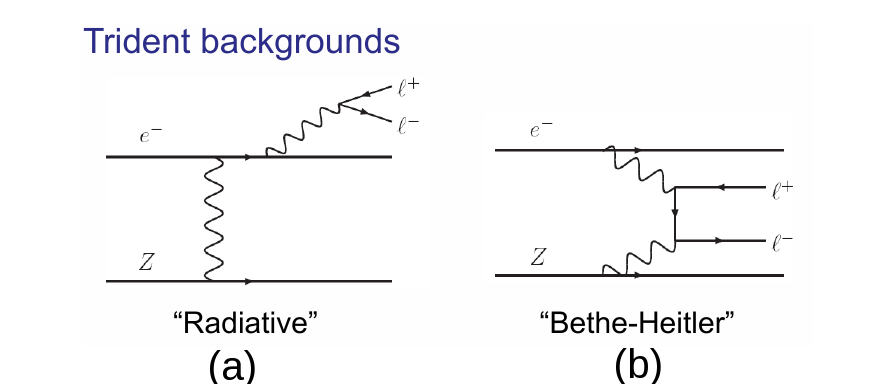
\includegraphics[width=.7\textwidth]{img/diagrams.png}
\caption{\label{fig:diagrams} Tree-level diagrams of radiative trident ($\gamma^*$) Bethe-Heitler trident reactions that comprise the primary background to the $A^\prime$ search.}
\end{figure}

\section{Benchmark framework}

In order to compare results from the different numerical codes listed before, a common benchmark framework was developed. Here, we list the general choices that were adopted, postponing a discussion to the specific implementation for each code in the following.
\begin{itemize}
\item The $W$ nucleus was parametrized as a spin 1/2 particle, with mass $M_W=171.25$ GeV. The lagrangian density for the $N-\gamma-N$ vertex thus reads (without the form-factor):
\begin{equation}
\mathcal{L}=-eA^\mu\,\overline{\psi}_N\gamma_\mu{\psi_N}
\end{equation}
\item The nuclear electromagnetic vertex is characterized by the following $G_2$ form-factor, that multiplies the \textit{amplitude} \cite{Bjorken:2009mm}: 
\begin{eqnarray}
%&G_{2,el}&=&\left( \frac{a^2t}{1+a^2t}\right)^2 \left(\frac{1}{1+t/d}\right)^2 Z^2  \nonumber \\
G_{2,el}&=&\frac{9Z^2}{(qR)^6}(\sin(qR)-qR\cos(qR))^2\nonumber \\
G_{2,in}&=& \left( \frac{{a^\prime}^2|t|}{1+{a^\prime}^2|t|}\right)^2 \left( \frac{1+\frac{|t|}{4m_p^2}(\mu^2_p-1)}{(1+|t|/D)^4} \right) Z\nonumber \\
G_2 &=& \sqrt{G_{2,el}+G_{2,in}} \; \; ,
\end{eqnarray}
where $t=(p_N - p_N^\prime)^2$ is the 4-momentum transferred to the nucleus, $q=\sqrt{-t}$, $Z=74$ and $A=183.84$ are the $W$ charge and mass, $R\simeq 1.2 \mbox{ fm }A^\frac{1}{3}$ is the $W$ radius in the model where the nucleus is an uniform sphere, $m_p$ is the proton mass, $\mu_p=2.79$, and $a^\prime=773 Z^{-2/3}/m_e$. By taking $m_p=0.9383$ GeV and $m_e=0.511\cdot 10^{-3}$ GeV, the following values are obtained. %These have been introduced in all the numerical codes that have been evaluated:
\begin{table}[H]
\centering
\begin{tabular}{|c|c|}
\hline
\textbf{Parameter}&\textbf{Value}\\
\hline
$R$ & 6.88 fm \\
\hline
$a^\prime$ & 85823.1 GeV$^{-1}$ \\
\hline
$D$ & 0.71 GeV$^2$ \\
\hline
\end{tabular}
\caption{Numerical values of the parameters entering the form-factor expression.}
\end{table}

\item The following cuts were employed in the calculation of the total cross-section and in the generation of Montecarlo unweighted events:
\begin{itemize}
\item $E_{e^-} > 0.05$ GeV,  $\theta^y_{e^-} > 0.01$ rad
\item $E_{e^+} > 0.05$ GeV, $\theta^y_{e^+} > 0.01$ rad
\item $E_{e^-}+E_{e^+} > 0.5$ GeV, $(P_{e^-}+P_{e^+})^2 > (0.01 \, \mbox{GeV})^2$ \; \; ,
\end{itemize}
where $E_{e^-}$ ($E_{e^+}$) is the electron (positron) energy in the laboratory frame, and $\theta^y_{e^-}$ ($\theta^y_{e^+}$) is the electron angle with respect to the primary beam axis ($z$), projected to the $yz$ plane.

The first cut on electron variables is satisfied if at least one of the two electrons passes it. The cut on the pair is satisfied if at least one of the two electrons, combined with the positron, passes it.

\end{itemize}

In the following, we report critical aspects in the implementation of the cross-section calculations specific to each code we used.

\subsection{MadGraph5}

The ``standard'' MadGraph5 packages included in the \texttt{hps-mc} distribution were used. 

\subsection{CalcHEP}

The calculation was performed modifying Standard Model to include the nucleus as a new particle, and implementing the corresponding interaction with photons. In the model, the value of the fine-structure constant was fixed to $\frac{1}{137}$.
The $W-\gamma-W$ form-factor has been implemented as an external function written in the \texttt{usrFF.c} file, that was then linked to the main application. Kinematic cuts were implemented using CalcHEP built-in kinematic functions.
Since the code doesn't allow to define $\theta^y$ and to cut on it, the selection on this variable was applied a-posteriori on the unweighted MonteCarlo events, and the total cross-section was properly scaled to account for this.

For each simulation run, the calculation was performed as follows. First, 25 cycles, each with $N_1=1\cdot 10^6$ calls, were performed to adapt the Vegas grid~\cite{vegas}. Then, 10 cycles with fixed grid, each with $N_2=1\cdot10^6$ calls, were performed to actually generated unweighted events and obtain the integrated cross-section.

\section{Radiative trident production}
To simplify the calculation, the ``reduced-interference'' approximation is used: the recoiling $e^-$ and the $e^-$ from pair production are assumed to be \textit{distinguishable}. Only the final state $e^-$ from pair production was considered when applying kinematic cuts\footnote{The use of the ``reduced-interference'' approximation is also required by the fact that CalcHEP, in case of identical particles in the final state, doesn't support the use of kinematic cuts applied to one of them only.}. 

Results of the comparison are shown in Fig.~\ref{fig:rad-xsec} and Fig.~\ref{fig:rad-kin}. Fig.~\ref{fig:rad-xsec} shows the total cross-section, integrated over the phase-space volume delimited by kinematic cuts. The two histograms refer respectively to MG5 (black) and to CalcHep (red). Each entry in the histogram is obtained from an independent calculation run. In each case, 500 calculation runs were performed. The result of a best-fit with a gaussian function to each distribution is shown in the same plot\footnote{In case of MadGraph5 distribution, featuring an asymmetric tail toward low $\sigma$ values, the fit to the histogram was performed starting from the mean value minus one standard deviation.}. The two average values for the total cross-section read:
\begin{itemize}
\item MG5: $4.495\pm0.002 \, \cdot 10^7$ pbarn
\item CalcHep: $4.391\pm0.008 \, \cdot 10^7$ pbarn
\end{itemize}
The CalcHep result is smaller with respect to the MG5 one by $\simeq 2\%$. Furthermore, the distribution of individual results obtained from the different calculation runs show a much larger width, possibly symptomatic of a slower convergence of the numerical procedure.

Fig.~\ref{fig:rad-kin}, instead, shows the kinematic distribution of final state particles, in terms of the total energy of the $e^+ e^-$ pair and of the corresponding invariant mass. Each distribution was obtained by computing the distribution in each calculation run and averaging them, including the corresponding total-cross section weight. The distributions obtained from MG5 and CalcHep show almost the same behavior.



\begin{figure}[tpb]
\centering
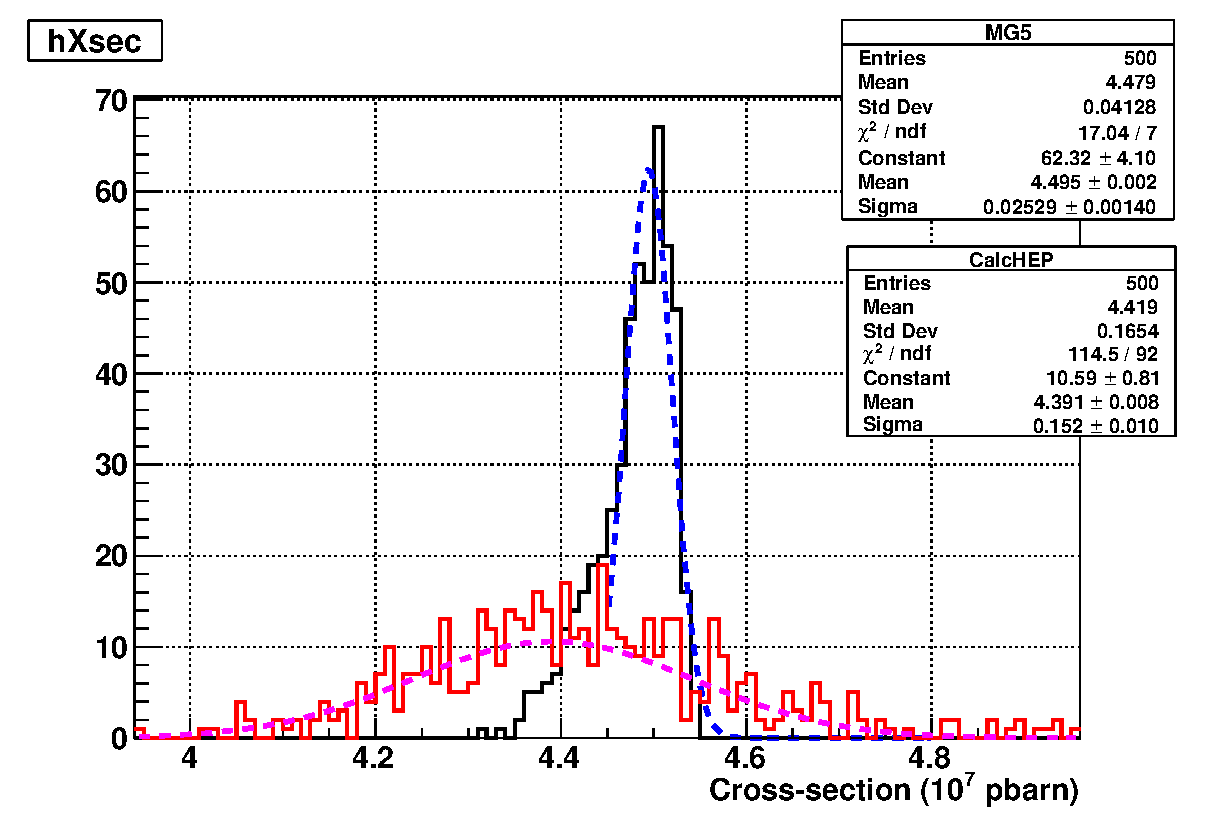
\includegraphics[width=.8\textwidth]{img/RAD_xsec.eps}
\caption{\label{fig:rad-xsec} \textbf{Radiative trident production (reduced interference):} total cross-section. Black: MG5, Red: CalcHep.}
\end{figure}

\begin{figure}[tpb]
\centering
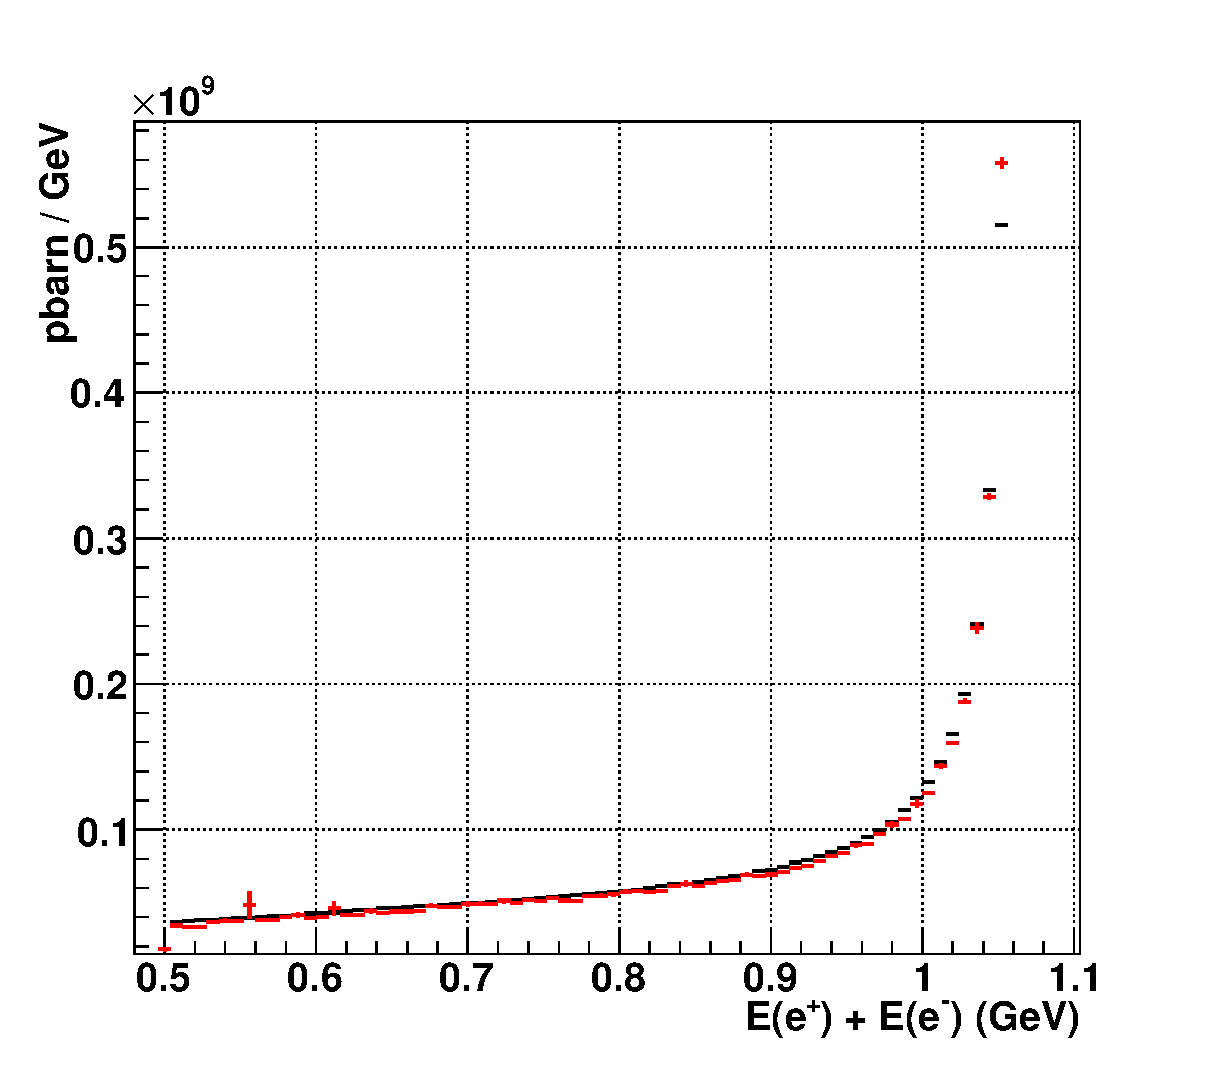
\includegraphics[width=.48\textwidth]{img/RAD_esum.eps}
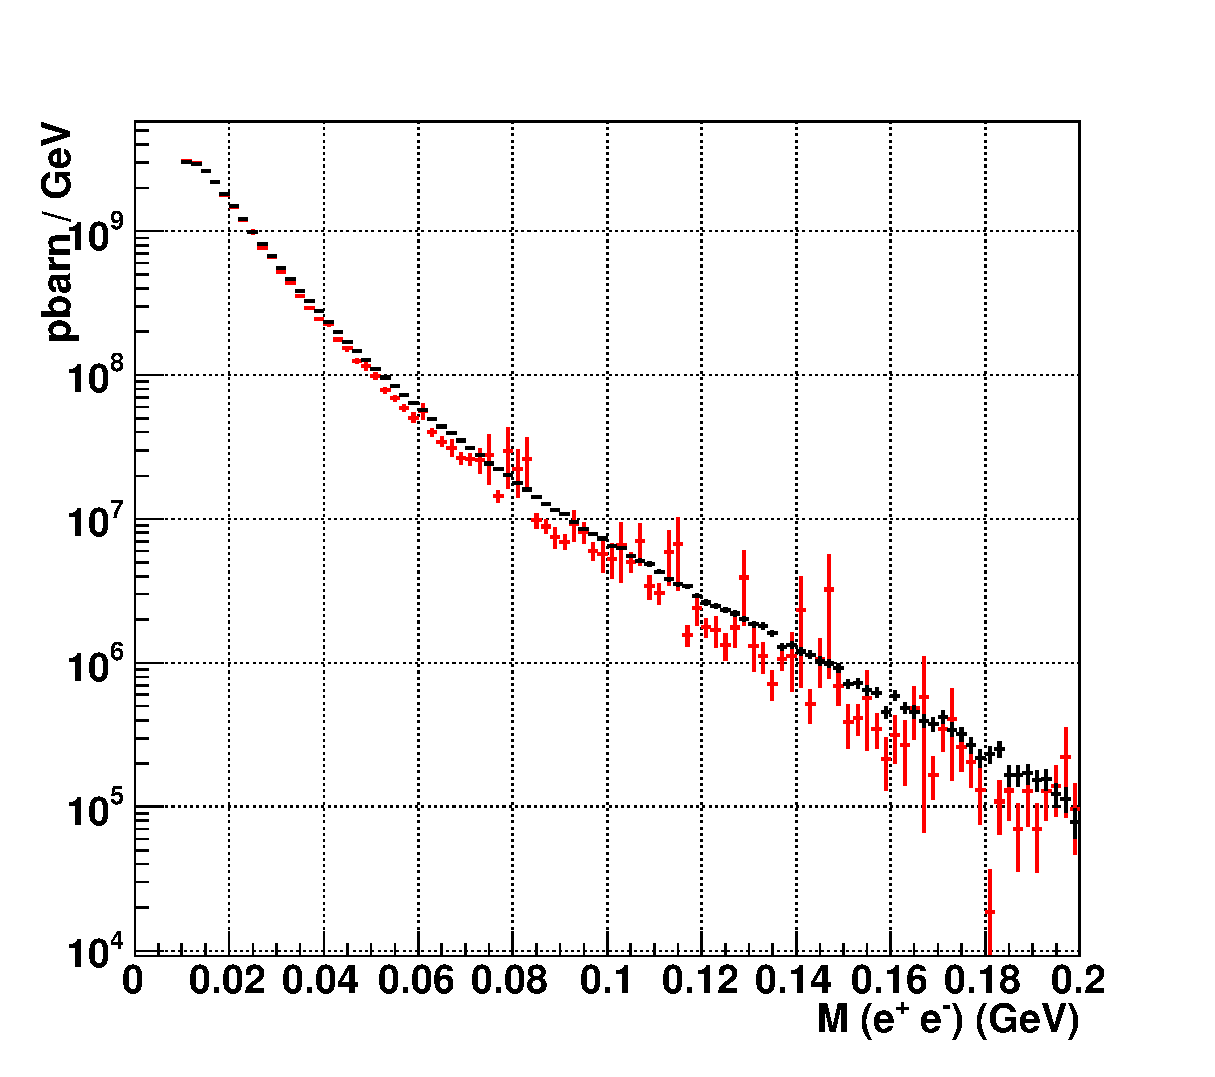
\includegraphics[width=.48\textwidth]{img/RAD_mass.eps}
\caption{\label{fig:rad-kin} \textbf{Radiative trident production (reduced interference):} kinematic distribution of events (black: MG5, red: CalcHep). Left: total energy of the $e^+ e^-$ pair. Right: invariant mass of the $e^+ e^-$ pair.}
\end{figure}


\section{Bethe-Heitler production}
To simplify the calculation, the ``reduced-interference'' approximation is used: the recoiling $e^-$ and the $e^-$ from pair production are assumed to be \textit{distinguishable}. Only the final state $e^-$ from pair production was considered when applying kinematic cuts.


Results of the comparison are shown in Fig.~\ref{fig:bh-xsec} and Fig.~\ref{fig:bh-kin}. Fig.~\ref{fig:bh-xsec} shows the total cross-section, integrated over the phase-space volume delimited by kinematic cuts (black:MG5, red:CalcHep). The two average values for the total cross-section read:
\begin{itemize}
\item MG5: $53.55\pm0.01 \, \cdot 10^7$ pbarn
\item CalcHep: $51.68\pm0.09 \, \cdot 10^7$ pbarn
\end{itemize}
As in the case of radiative trident production, the CalcHep result is smaller with respect to the MG5. The difference is $\simeq 3.5\%$. Again, the distribution of individual results obtained from the different calculation runs show a much larger width, possibly symptomatic of a slower convergence of the numerical procedure.


\begin{figure}[tpb]
\centering
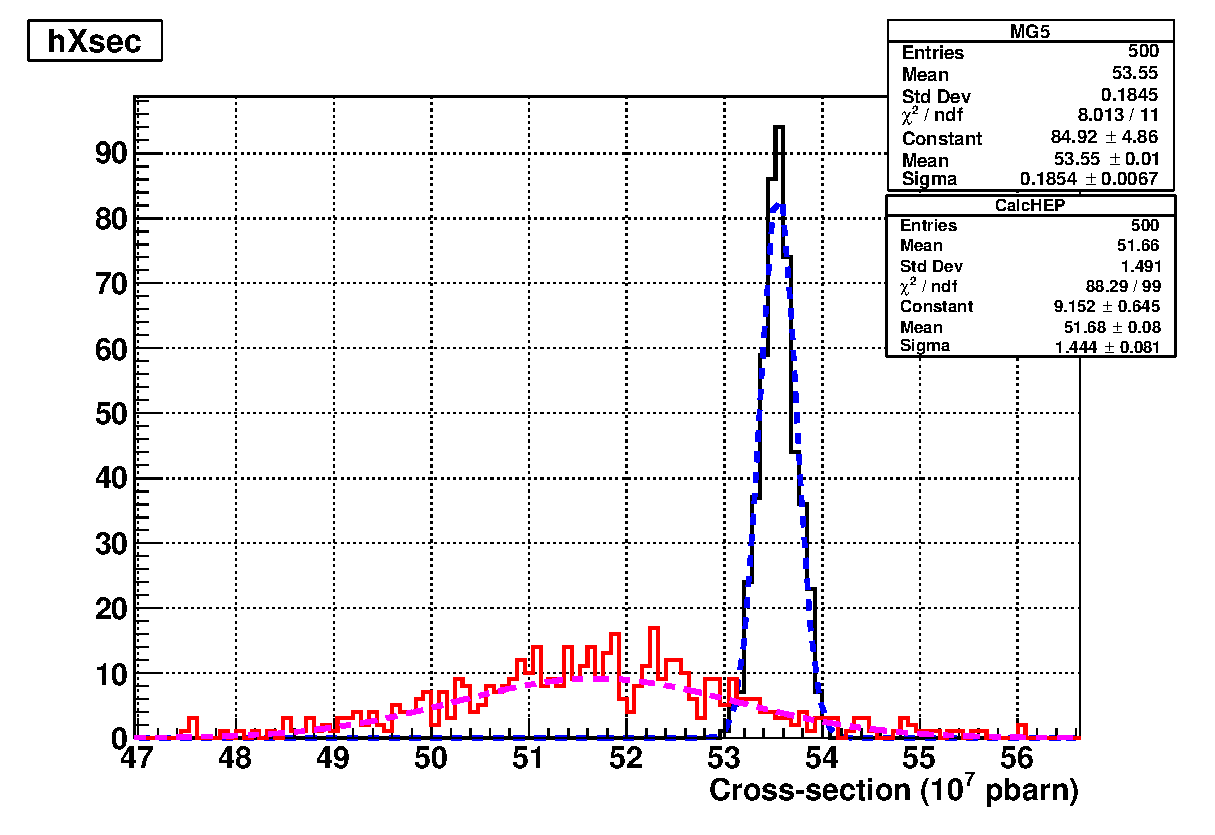
\includegraphics[width=.8\textwidth]{img/BH_xsec.eps}
\caption{\label{fig:bh-xsec} \textbf{Bethe-Heitler trident production (reduced interference):} total cross-section. Black: MG5, Red: CalcHep.}
\end{figure}

\begin{figure}[tpb]
\centering
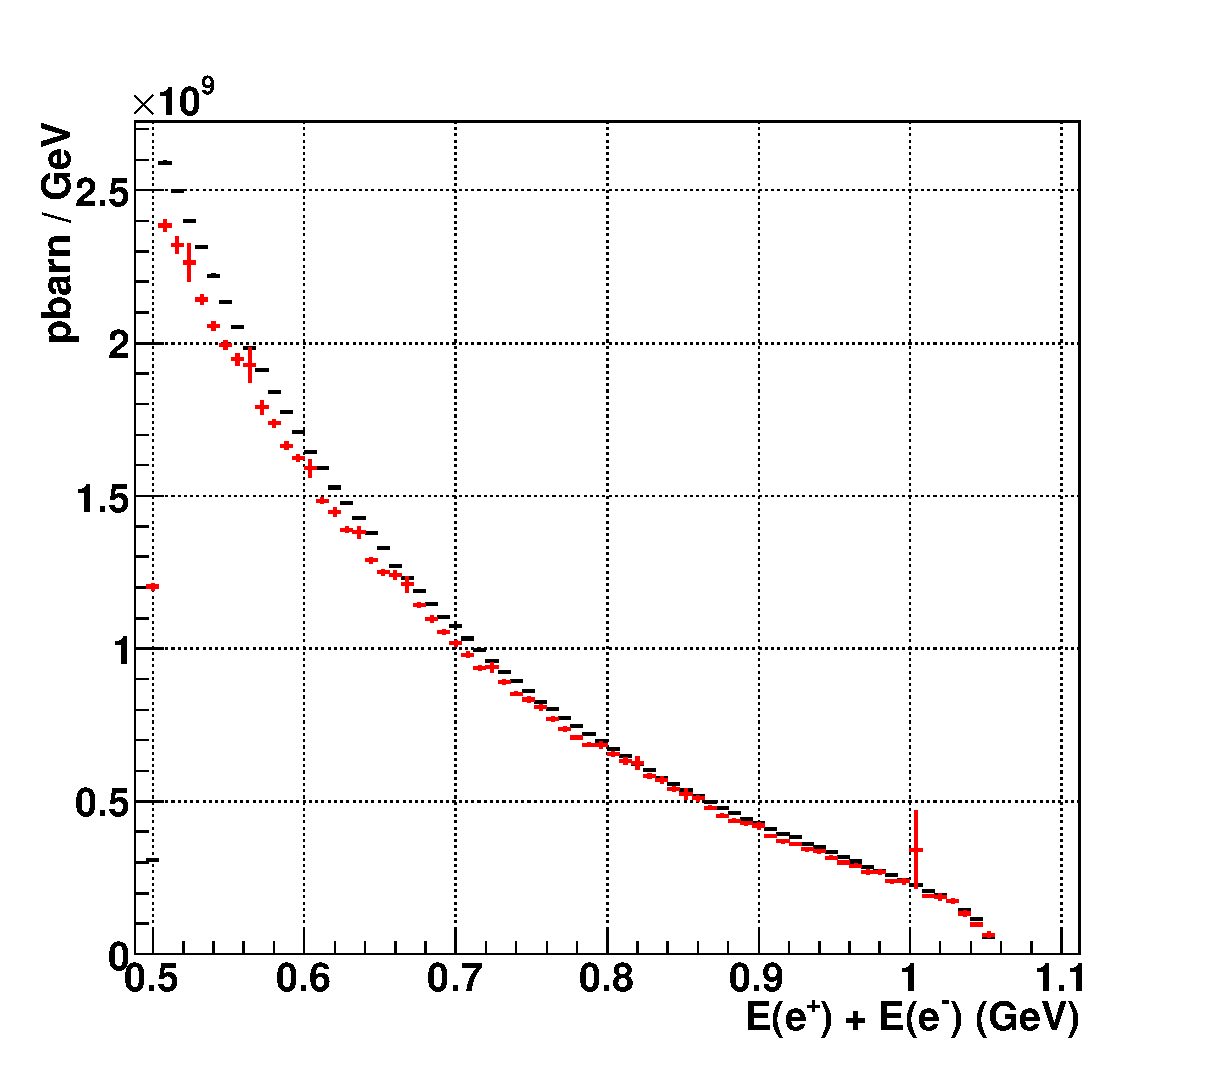
\includegraphics[width=.48\textwidth]{img/BH_esum.eps}
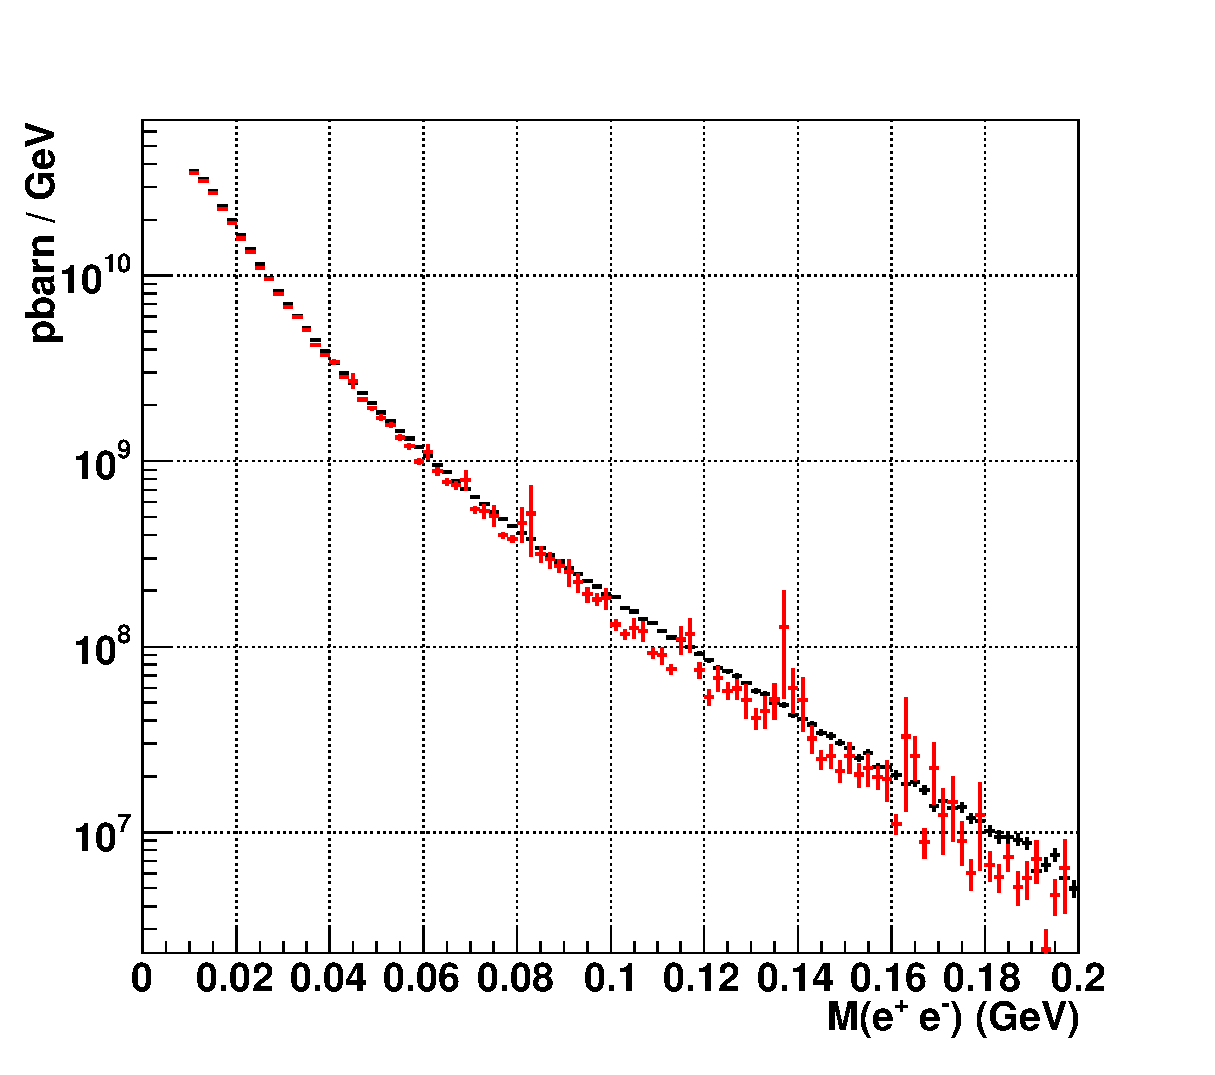
\includegraphics[width=.48\textwidth]{img/BH_mass.eps}
\caption{\label{fig:bh-kin} \textbf{Bethe-Heitler trident production (reduced interference):} kinematic distribution of events (black: MG5, red: CalcHep). Left: total energy of the $e^+ e^-$ pair. Right: invariant mass of the $e^+ e^-$ pair.}
\end{figure}

Fig.~\ref{fig:bh-kin}, instead, shows the kinematic distribution of final state particles, in terms of the total energy of the $e^+ e^-$ pair and of the corresponding invariant mass. Each distribution was obtained by computing the distribution in each calculation run and averaging them, including the corresponding total-cross section weight. The distributions obtained from MG5 and CalcHep show a similar behavior. For low total energy values, the CalcHep differential cross-section is smaller than the MadGraph one by a factor of about $10\%$, the difference becoming smaller for larger values of the total energy.

\section{Conclusions}

We compared results obtained from CalcHep and MadGraph5 in calculating the total cross-section and the kinematic distribution of events for the Radiative and Bethe-Heitler trident electro-production on a nuclear target. The calculation was performed in the ``reduced-interference'' approximation. Each calculation was performed 500 times. Results show that the total cross-sections are different by $2\%$ (Radiative) - $3.5\%$ (Bethe-Heitler), with the CalcHep result being smaller than the MG5 one in each case. Furthermore, the CalcHep distribution show a much larger width - possibly symptomatic of a slower convergence of this numerical procedure.

Kinematic distributions for the total energy of the $e^+ e^-$ pair and for the corresponding invariant mass were also compared, in terms of the corresponding differential cross-section. For both processes, the two exhibit the same shape. In case of Bethe-Heitler production, the CalcHep under-estimate of the total cross-section reflects in the total-energy differential cross-section to be smaller than the corresponding MadGraph result for low values of this variable, close to $E(e^+)+E(e^-) = 0.5$ GeV.


 \begin{thebibliography}{1}

  %\bibitem{notes} John W. Dower {\em Readings compiled for History 21.479.}  1991.
 \bibitem{Alwall:2011uj} 
  J.~Alwall, M.~Herquet, F.~Maltoni, O.~Mattelaer and T.~Stelzer,
  %``MadGraph 5 : Going Beyond,''
  JHEP {\bf 1106}, 128 (2011)
  doi:10.1007/JHEP06(2011)128
  [arXiv:1106.0522 [hep-ph]].
  %%CITATION = doi:10.1007/JHEP06(2011)128;%%
  %2641 citations counted in INSPIRE as of 16 May 2018
%\cite{Belyaev:2012qa}
\bibitem{Belyaev:2012qa} 
  A.~Belyaev, N.~D.~Christensen and A.~Pukhov,
  %``CalcHEP 3.4 for collider physics within and beyond the Standard Model,''
  Comput.\ Phys.\ Commun.\  {\bf 184}, 1729 (2013)
  doi:10.1016/j.cpc.2013.01.014
  [arXiv:1207.6082 [hep-ph]].
  %%CITATION = doi:10.1016/j.cpc.2013.01.014;%%
  %524 citations counted in INSPIRE as of 16 May 2018

\bibitem{Bjorken:2009mm} 
  J.~D.~Bjorken, R.~Essig, P.~Schuster and N.~Toro,
  %``New Fixed-Target Experiments to Search for Dark Gauge Forces,''
  Phys.\ Rev.\ D {\bf 80}, 075018 (2009)
  doi:10.1103/PhysRevD.80.075018
  [arXiv:0906.0580 [hep-ph]].
  %%CITATION = doi:10.1103/PhysRevD.80.075018;%%
  %422 citations counted in INSPIRE as of 16 May 2018


\bibitem{vegas} 
  T.~Ohl,
  %``Vegas revisited: Adaptive Monte Carlo integration beyond factorization,''
  Comput.\ Phys.\ Commun.\  {\bf 120}, 13 (1999)
  doi:10.1016/S0010-4655(99)00209-X
  [hep-ph/9806432].
  %%CITATION = doi:10.1016/S0010-4655(99)00209-X;%%
  %78 citations counted in INSPIRE as of 24 May 2018


  \end{thebibliography}
\end{document}
